\documentclass{standalone}
\usepackage{tikz}
\usetikzlibrary{patterns, positioning}


\begin{document}
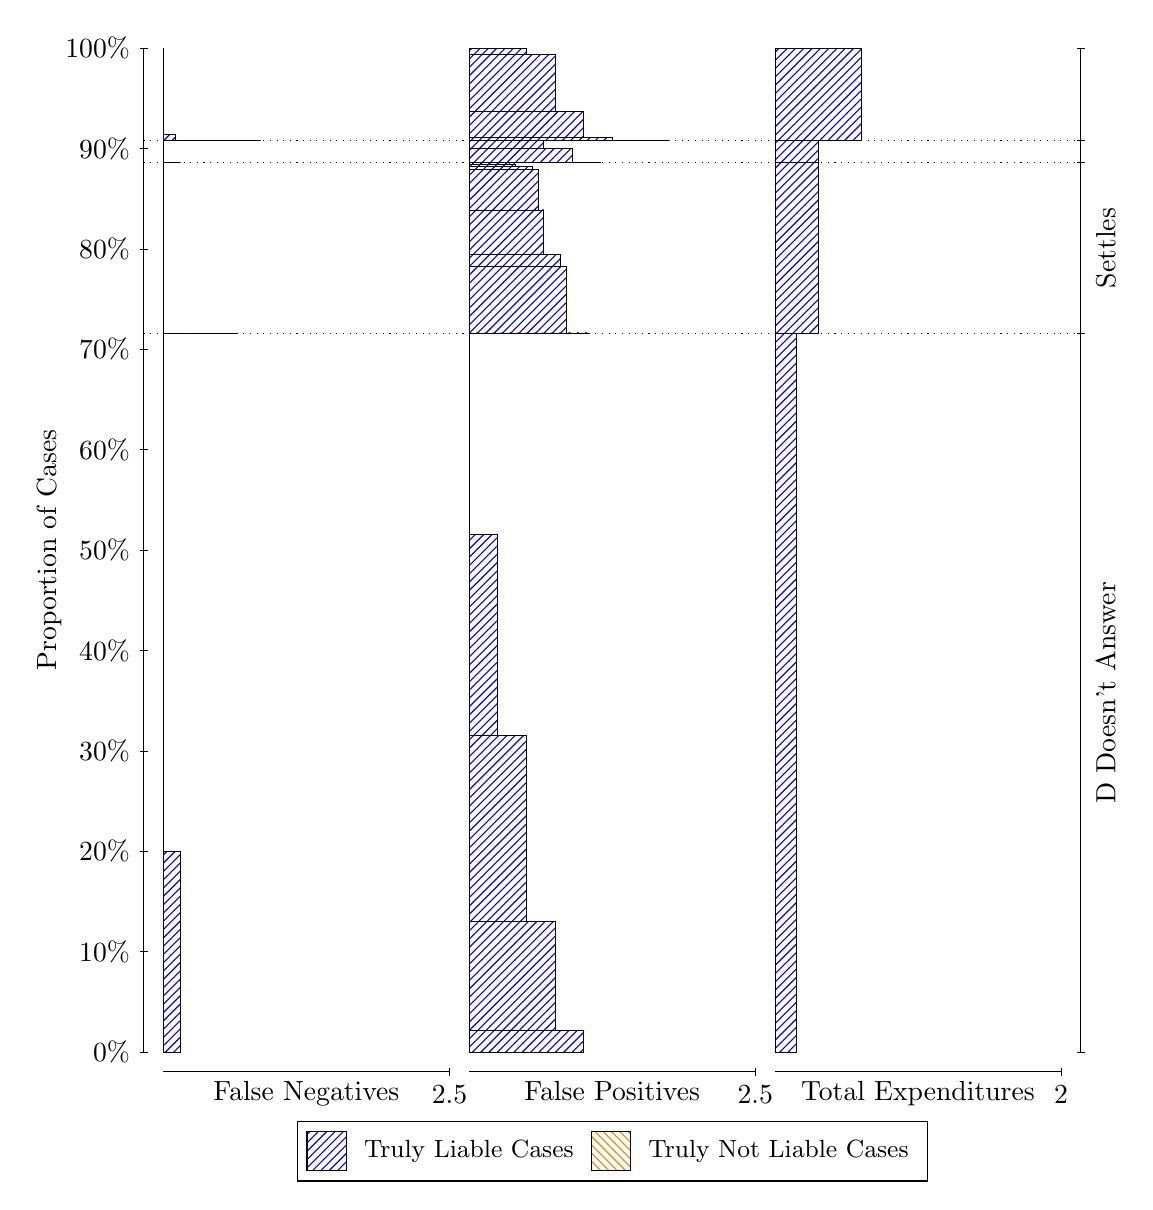
\begin{tikzpicture}
\draw[black, very thin] (1.5,1.75) -- (1.5,14.5);
\node[rotate=90, text=black, anchor=center] at (0.3, 8.125) {Proportion of Cases};
\draw[black, very thin] (1.45,1.75) -- (1.55,1.75);
\node[text=black, anchor=east] at (1.45, 1.75) {0\%};
\draw[black, very thin] (1.45,3.025) -- (1.55,3.025);
\node[text=black, anchor=east] at (1.45, 3.025) {10\%};
\draw[black, very thin] (1.45,4.3) -- (1.55,4.3);
\node[text=black, anchor=east] at (1.45, 4.3) {20\%};
\draw[black, very thin] (1.45,5.575) -- (1.55,5.575);
\node[text=black, anchor=east] at (1.45, 5.575) {30\%};
\draw[black, very thin] (1.45,6.85) -- (1.55,6.85);
\node[text=black, anchor=east] at (1.45, 6.85) {40\%};
\draw[black, very thin] (1.45,8.125) -- (1.55,8.125);
\node[text=black, anchor=east] at (1.45, 8.125) {50\%};
\draw[black, very thin] (1.45,9.4) -- (1.55,9.4);
\node[text=black, anchor=east] at (1.45, 9.4) {60\%};
\draw[black, very thin] (1.45,10.675) -- (1.55,10.675);
\node[text=black, anchor=east] at (1.45, 10.675) {70\%};
\draw[black, very thin] (1.45,11.95) -- (1.55,11.95);
\node[text=black, anchor=east] at (1.45, 11.95) {80\%};
\draw[black, very thin] (1.45,13.225) -- (1.55,13.225);
\node[text=black, anchor=east] at (1.45, 13.225) {90\%};
\draw[black, very thin] (1.45,14.5) -- (1.55,14.5);
\node[text=black, anchor=east] at (1.45, 14.5) {100\%};

\draw[black, very thin] (13.4,1.75) -- (13.4,14.5);
\draw[black, very thin] (13.35,1.75) -- (13.45,1.75);
\node[anchor=west] at (13.35, 1.75) {};
\draw[black, very thin] (13.35,10.873) -- (13.45,10.873);
\node[anchor=west] at (13.35, 10.873) {};
\draw[black, very thin] (13.35,13.046) -- (13.45,13.046);
\node[anchor=west] at (13.35, 13.046) {};
\draw[black, very thin] (13.35,13.328) -- (13.45,13.328);
\node[anchor=west] at (13.35, 13.328) {};
\draw[black, very thin] (13.35,14.5) -- (13.45,14.5);
\node[anchor=west] at (13.35, 14.5) {};

\draw[black, very thin, pattern color=blue, pattern=north east lines] (1.75,1.75) rectangle (1.968,4.2999);
\draw[black, very thin, pattern color=orange, pattern=north west lines] (1.75,4.2999) rectangle (1.75,4.2999);
\draw[black, very thin, pattern color=blue, pattern=north east lines] (1.75,4.2999) rectangle (1.75,10.873);
\draw[black, very thin, pattern color=blue, pattern=north east lines] (1.75,10.873) rectangle (2.6947,10.873);
\draw[black, very thin, pattern color=blue, pattern=north east lines] (1.75,10.873) rectangle (2.404,10.873);
\draw[black, very thin, pattern color=blue, pattern=north east lines] (1.75,10.873) rectangle (2.3313,10.873);
\draw[black, very thin, pattern color=blue, pattern=north east lines] (1.75,10.873) rectangle (2.1133,10.873);
\draw[black, very thin, pattern color=blue, pattern=north east lines] (1.75,10.873) rectangle (2.0407,10.873);
\draw[black, very thin, pattern color=blue, pattern=north east lines] (1.75,10.873) rectangle (1.968,10.873);
\draw[black, very thin, pattern color=orange, pattern=north west lines] (1.75,10.873) rectangle (1.75,10.873);
\draw[black, very thin, pattern color=blue, pattern=north east lines] (1.75,10.873) rectangle (1.75,13.046);
\draw[black, very thin, pattern color=blue, pattern=north east lines] (1.75,13.046) rectangle (1.968,13.046);
\draw[black, very thin, pattern color=orange, pattern=north west lines] (1.75,13.046) rectangle (1.75,13.046);
\draw[black, very thin, pattern color=blue, pattern=north east lines] (1.75,13.046) rectangle (1.75,13.328);
\draw[black, very thin, pattern color=blue, pattern=north east lines] (1.75,13.328) rectangle (2.9853,13.328);
\draw[black, very thin, pattern color=blue, pattern=north east lines] (1.75,13.328) rectangle (2.622,13.328);
\draw[black, very thin, pattern color=blue, pattern=north east lines] (1.75,13.328) rectangle (2.2587,13.328);
\draw[black, very thin, pattern color=blue, pattern=north east lines] (1.75,13.328) rectangle (2.2587,13.329);
\draw[black, very thin, pattern color=blue, pattern=north east lines] (1.75,13.329) rectangle (1.8953,13.329);
\draw[black, very thin, pattern color=blue, pattern=north east lines] (1.75,13.329) rectangle (1.8953,13.405);
\draw[black, very thin, pattern color=orange, pattern=north west lines] (1.75,13.405) rectangle (1.75,13.405);
\draw[black, very thin, pattern color=blue, pattern=north east lines] (1.75,13.405) rectangle (1.75,14.5);
\draw[black, very thin, pattern color=orange, pattern=north west lines] (5.6333,1.75) rectangle (7.0867,1.75);
\draw[black, very thin, pattern color=blue, pattern=north east lines] (5.6333,1.75) rectangle (7.0867,2.0215);
\draw[black, very thin, pattern color=blue, pattern=north east lines] (5.6333,2.0215) rectangle (6.7233,3.4044);
\draw[black, very thin, pattern color=blue, pattern=north east lines] (5.6333,3.4044) rectangle (6.36,5.7749);
\draw[black, very thin, pattern color=blue, pattern=north east lines] (5.6333,5.7749) rectangle (5.9967,8.3234);
\draw[black, very thin, pattern color=blue, pattern=north east lines] (5.6333,8.3234) rectangle (5.6333,10.873);
\draw[black, very thin, pattern color=orange, pattern=north west lines] (5.6333,10.873) rectangle (7.1593,10.873);
\draw[black, very thin, pattern color=blue, pattern=north east lines] (5.6333,10.873) rectangle (7.1593,10.882);
\draw[black, very thin, pattern color=orange, pattern=north west lines] (5.6333,10.882) rectangle (6.8687,10.882);
\draw[black, very thin, pattern color=blue, pattern=north east lines] (5.6333,10.882) rectangle (6.8687,11.73);
\draw[black, very thin, pattern color=blue, pattern=north east lines] (5.6333,11.73) rectangle (6.796,11.877);
\draw[black, very thin, pattern color=orange, pattern=north west lines] (5.6333,11.877) rectangle (6.578,11.877);
\draw[black, very thin, pattern color=blue, pattern=north east lines] (5.6333,11.877) rectangle (6.578,12.445);
\draw[black, very thin, pattern color=blue, pattern=north east lines] (5.6333,12.445) rectangle (6.5053,12.959);
\draw[black, very thin, pattern color=blue, pattern=north east lines] (5.6333,12.959) rectangle (6.4327,13.001);
\draw[black, very thin, pattern color=blue, pattern=north east lines] (5.6333,13.001) rectangle (6.2147,13.029);
\draw[black, very thin, pattern color=blue, pattern=north east lines] (5.6333,13.029) rectangle (6.142,13.045);
\draw[black, very thin, pattern color=blue, pattern=north east lines] (5.6333,13.045) rectangle (6.0693,13.046);
\draw[black, very thin, pattern color=blue, pattern=north east lines] (5.6333,13.046) rectangle (5.8513,13.046);
\draw[black, very thin, pattern color=blue, pattern=north east lines] (5.6333,13.046) rectangle (5.7787,13.046);
\draw[black, very thin, pattern color=blue, pattern=north east lines] (5.6333,13.046) rectangle (5.706,13.046);
\draw[black, very thin, pattern color=blue, pattern=north east lines] (5.6333,13.046) rectangle (5.6333,13.046);
\draw[black, very thin, pattern color=orange, pattern=north west lines] (5.6333,13.046) rectangle (7.3047,13.046);
\draw[black, very thin, pattern color=blue, pattern=north east lines] (5.6333,13.046) rectangle (7.3047,13.052);
\draw[black, very thin, pattern color=blue, pattern=north east lines] (5.6333,13.052) rectangle (6.9413,13.224);
\draw[black, very thin, pattern color=blue, pattern=north east lines] (5.6333,13.224) rectangle (6.578,13.327);
\draw[black, very thin, pattern color=blue, pattern=north east lines] (5.6333,13.327) rectangle (6.2147,13.328);
\draw[black, very thin, pattern color=blue, pattern=north east lines] (5.6333,13.328) rectangle (5.8513,13.328);
\draw[black, very thin, pattern color=orange, pattern=north west lines] (5.6333,13.328) rectangle (8.1767,13.328);
\draw[black, very thin, pattern color=blue, pattern=north east lines] (5.6333,13.328) rectangle (8.1767,13.328);
\draw[black, very thin, pattern color=orange, pattern=north west lines] (5.6333,13.328) rectangle (7.8133,13.328);
\draw[black, very thin, pattern color=blue, pattern=north east lines] (5.6333,13.328) rectangle (7.8133,13.329);
\draw[black, very thin, pattern color=orange, pattern=north west lines] (5.6333,13.329) rectangle (7.45,13.329);
\draw[black, very thin, pattern color=blue, pattern=north east lines] (5.6333,13.329) rectangle (7.45,13.362);
\draw[black, very thin, pattern color=orange, pattern=north west lines] (5.6333,13.362) rectangle (7.0867,13.362);
\draw[black, very thin, pattern color=blue, pattern=north east lines] (5.6333,13.362) rectangle (7.0867,13.698);
\draw[black, very thin, pattern color=orange, pattern=north west lines] (5.6333,13.698) rectangle (6.7233,13.698);
\draw[black, very thin, pattern color=blue, pattern=north east lines] (5.6333,13.698) rectangle (6.7233,14.423);
\draw[black, very thin, pattern color=blue, pattern=north east lines] (5.6333,14.423) rectangle (6.36,14.5);
\draw[black, very thin, pattern color=blue, pattern=north east lines] (5.6333,14.5) rectangle (5.9967,14.5);
\draw[black, very thin, pattern color=blue, pattern=north east lines] (5.6333,14.5) rectangle (5.6333,14.5);
\draw[black, very thin, pattern color=orange, pattern=north west lines] (9.5167,1.75) rectangle (9.7892,1.75);
\draw[black, very thin, pattern color=blue, pattern=north east lines] (9.5167,1.75) rectangle (9.7892,10.873);
\draw[black, very thin, pattern color=orange, pattern=north west lines] (9.5167,10.873) rectangle (10.062,10.873);
\draw[black, very thin, pattern color=blue, pattern=north east lines] (9.5167,10.873) rectangle (10.062,13.046);
\draw[black, very thin, pattern color=orange, pattern=north west lines] (9.5167,13.046) rectangle (10.062,13.046);
\draw[black, very thin, pattern color=blue, pattern=north east lines] (9.5167,13.046) rectangle (10.062,13.328);
\draw[black, very thin, pattern color=orange, pattern=north west lines] (9.5167,13.328) rectangle (10.607,13.328);
\draw[black, very thin, pattern color=blue, pattern=north east lines] (9.5167,13.328) rectangle (10.607,14.5);
\draw[black, dotted] (1.5,10.873) -- (13.4,10.873);
\draw[black, dotted] (1.5,13.046) -- (13.4,13.046);
\draw[black, dotted] (1.5,13.328) -- (13.4,13.328);
\draw[black, very thin] (1.75,1.5) -- (5.3833,1.5);
\node[text=black, anchor=north] at (3.5667, 1.5) {False Negatives};
\draw[black, very thin] (5.3833,1.45) -- (5.3833,1.55);
\node[text=black, anchor=north] at (5.3833, 1.45) {2.5};

\draw[black, very thin] (5.6333,1.5) -- (9.2667,1.5);
\node[text=black, anchor=north] at (7.45, 1.5) {False Positives};
\draw[black, very thin] (9.2667,1.45) -- (9.2667,1.55);
\node[text=black, anchor=north] at (9.2667, 1.45) {2.5};

\draw[black, very thin] (9.5167,1.5) -- (13.15,1.5);
\node[text=black, anchor=north] at (11.333, 1.5) {Total Expenditures};
\draw[black, very thin] (13.15,1.45) -- (13.15,1.55);
\node[text=black, anchor=north] at (13.15, 1.45) {2};

\node[text=black, centered, rotate=90] at (13.72, 6.3117) {D Doesn't Answer};
\node[text=black, centered, rotate=90] at (13.72, 11.959) {Settles};



\draw (7.449999999999999,1.5) node[draw=none] (baseCoordinate) {};
\begin{scope}[align=center]
        \matrix[scale=0.5, draw=black, below=0.5cm of baseCoordinate, nodes={draw}, column sep=0.1cm]{
            \node[rectangle, draw, minimum width=0.5cm, minimum height=0.5cm, pattern color=blue, pattern=north east lines] {}; &
            \node[draw=none, font=\small, text=black] (B) {Truly Liable Cases}; &
            \node[rectangle, draw, minimum width=0.5cm, minimum height=0.5cm, pattern color=orange, pattern=north west lines] {}; &
            \node[draw=none, font=\small, text=black] (B) {Truly Not Liable Cases}; \\
            };
\end{scope}

\end{tikzpicture}
\end{document}